%----------------------------------------------------------------------------
\chapter*{Bevezető}\addcontentsline{toc}{chapter}{Bevezető}
%----------------------------------------------------------------------------

A programozói ismeretek elsajátításához merőben más módszertanra van szükség, mint egy irodalmi vagy jogász pályán. Az előbbi előnye, hogy megfelelő háttér biztosításával nagyban javítható a tanulási görbe, azonban sajnos az egyetemi körülmények között nincs lehetőség minden halltóval személyesen foglalkozni, hiszen ez óriási többlet munkát róna az oktatókra. Emiatt a hallgatók eredményes, mégis időtakarékos támogatása érdekében egyre nagyobb törekvés indult az automatizálása felé. Ezen megoldások számos előnnyel rendelkezhetnek:

\begin{itemize}
    \item Az értékeléshez nincs szükség a beadások letöltésére, azok saját számítógépen történő fordítására, futtatására, majd kiértékelésére.
    \item Azonnali visszajelzés a beadás sikerességéről a hallgatóknak.
    \item Egyéb beadáshoz kapcsolható metrikákkal is dolgohatunk: futási idő, memóriahasználat, stb.
    \item Automatikus pontszámítás a számított metrikák alapján.
    \item Határidők automatikus kezelése.
    \item Kommunikációs felület a hallgató és oktató között.
\end{itemize}

Természetesen egy-egy ilyen szoftver elkészítésénél cél az előbbi előnyök legnagyobb mértékű teljesítése, illetve kiegészítése a lokálisan tapasztalt további igényekkel.

\section*{A szakdolgozat felépítése}\addcontentsline{toc}{section}{A szakdolgozat felépítése}
A szakdolgozatom \ref{chapter:othersystems}. fejezetében bemutatom a JPorta rendszeréhez hasonló,  mindenki számára elérhető, nyílt forráskódú rendszereket. Majd \aref{chapter:jporta}. fejezetében ismertetem a JPorta felépítését és főbb funkcióit. Itt részletezem a nyújtott szolgáltatások elérését, a hallgatól által elérhető funkciók részleteit. Végül pedig kitérek a JPorta moduljainak kapcsolatára.

\aref{chapter:assessments}. fejezetben részletezem az értékelési rendszer funkcióit, kiemelve a dinamikus mezőket. Kitérek a dinamikus mezők jelenlegi implementációs részleteire, működésükre és tesztelhetőségükre. Ezután ismertetem a megoldásomat a dinamikus függőségek problémájának megoldására.

\aref{chapter:exercise}. fejezetben az automatizált feladatkiértékelő modul kelül az előtérbe, részletezem annak működését. Kitérek a jogosultság kezelés problémájára, ezek felülvizsgálatára. Ezután a beadott megoldások kódlefedettség ellenőrzésére készített modult ismertetem, végül pedig a felmerülő további lehetőségeket.

A szakdolgozatomat az elvégzett munka összefoglalásával zárom.

\chapter{eLearning rendszerek}\label{chapter:othersystems}

Az elmúlt években egyre hagsúlyosabbá vált az online oktatás annak előnyei miatt. Ennek eredményeképpen egyre több és több online kurzusokat biztosító és biztosítását lehetővé tévő weboldal jelent meg. \cite{eLearningPopularity}

Ezen weboldalak jelentős része mint szolgáltatás működik, azaz kurzusokat (ingyeneseket és/vagy csak térítés ellenében elérhetőeket) biztosítanak, de sokszor nem, vagy csak korlátozottan biztosítanak lehetőséget arra, hogy saját tanfolyamot indítsunk. Más portálok nyílt forráskódúak, melynek köszönhetően személyre szabhatóak és saját szerveren futtathatóak. Ennek előnye, hogy a kurzusunk nem függ más rendszerektől és mindent saját kézben tarthatunk.

\section{Moodle}
A Moodle \cite{Moodle} egy teljes körű eLearning rendszer, mely nyílt forráskódú GNU GPL \cite{GNUGPL} licenc alatt készült. A Moodle-nek mára több, mint 120 ezer felhasználója van, a világ 232 országában \cite{MoodleStats}, amivel ez az egyik legnépszerűbb eLearning rendszer.

A Moodle általános lehetőséget biztosít az online oktatáshoz. Egyszerűen hozhatunk létre benne kurzusokat, melyekre a jelentkezést akár korlátozhatjuk is. A kurzusokon belül témakörökre bonthatjuk a tananyagot, melynek formája sokféle lehet: pdf fájlok, videók, külső weboldalak, stb. A résztvevők elsajátított tudásának ellenőrzése sem marad el: a Moodle általános rendszert biztosít online tesztek készítésére is, különféle jelleggel, mint pl. több válaszlehetőségből helyes(ek) kiválasztása, egy soros vagy éppen hosszabb saját szavas válaszok. A legtöbb fajta tesztnél lehetőségünk van a helyes válaszok megadására, így a portál azonnal ki is értékeli a beadást, ennek köszönhetően pedig a felhasználó azonnal értesül az elért eredményéről.

\begin{figure}[h]
    \centering
    \resizebox{\textwidth}{!}{
        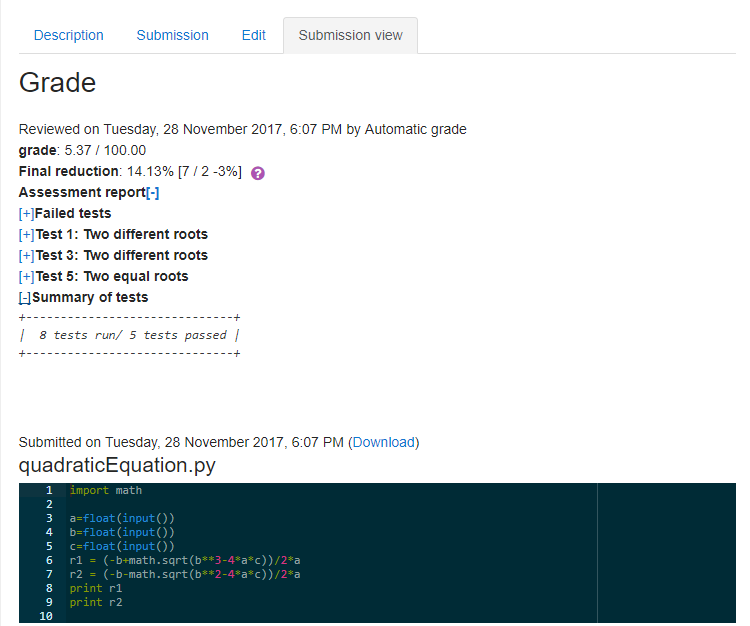
\includegraphics[]{moodle_vpl.png}
    }
    \caption{Moodle Virtual Programming Lab feladatbeadás}
    \label{fig:moodle_vpl}
\end{figure}

Elterjedtségének köszönhetően számos közösségi fejlesztésű modul is készült hozzá, melyek közül találhatunk szép számmal a programozás oktatására fókuszálókat is. Ilyen például a Virtual Programming Lab \cite{VPL} \cite{VPLJournal}, mely támogat forráskódszerkesztést a böngészőben, programok futtatását, ellenőrzését és plágium ellenőrzést is. Mindezt a felhasználók a már megszokott Moodle környezetben érhetik el a kényelmes használat érdekében.

\section{ATutor}

Az ATutor (\url{\checkmark/}) a Moodle-höz hasonló nyílt forráskódú eLearning rendszer. A tanultak ellenőrzésére több típusból álló tesztsor automatikus kiértékelését is támogatja. Ilyen kérdés típusok lehetnek helyes válaszok kiválasztása, igaz-hamis kérdések, sorbarendezések, stb. Ugyanakkor nincs beépített programozás oktatást támogató modulja, aminek segítségével a felhasználó programozási feladatait tudná automatikus ellenőriztetni a rendszerrel.

\section{edX, Open edX}
Az edX \cite{EDXAbout} egy nonprofit online kezdeményezés, melynek alapítói a Harvard University és a Massachusetts Institute of Technology. Ennek segítségével egyetemi szintű kurzusokat tartanak világszerte közel 10 millió felhasználóval és több, mint ezer kurzussal \cite{EDXReview}.

Az edX rendszer nem csak egyszerű tananyagok megtekintésére biztosít lehetőséget, de videókat és egyéb feladatokat is találunk a kínált kurzusokban. Emellett egyszerűen kapcsolatba léphetünk másokkal, akik a kurzusunkat hallgatják, ha éppen segítségre lenne szükségünk. A kurzusok többnyire ingyenesek, de sok esetben van lehetőségünk fizetés ellenében igazolást kapnunk a sikeresen elvégzett kurzusról.

A portálon lehetőségünk van programozással kapcsolatos kurzusok felvételére is. Ezek keretében pedig online kód írásra, fordításra, futtatásra és a helyesség ellenőrzésére is van mód, amik nélkül az önálló tanulás nagyon nehézkes lenne. Webes kódolást némely kurzusnál Codeboard\footnotemark integrációval van megoldva, melynek köszönhetően nem is kell a tanuláshoz a megfelelő környezeteket telepítenünk a saját gépünkre.
\footnotetext{A Codeboard (http://codeboard.io) egy böngésző alapú fejlesztő környezet a programozás oktatás segítésére. Támogatja az edX, moodle, cursera és egyéb platformokat.}

Az Open edX egy nyílt forráskódú platform, melyet az edX fejlesztett ki és tett szabadon hozzáférhetővé saját oktatási környezetek létrehozására. Közel a teljes szerver oldali kód Python nyelven íródott, melynek széleskörű ismerttségének (és a rendszer nyílt forráskódú voltának) köszönhetően bárki kiegészítheti a meglévő kódot.

\section{Codeacademy}

A Codeacademy (\url{https://www.codecademy.com}) az előzőekhez hasonlóan egy eLearning rendszer, amely felhasználói számára számos programnyelvhez kínál tanulási lehetőségeket, mint a Python, Java, PHP és JavaScript nyelvek. A weboldalon regisztráció után ingyenesen hozzáférhetünk a kurzusokhoz, de lehetőségünk van a Pro verziót is választani. Itt fizetés ellenében élő támogatást, tanulási egységenkénti ellenőrző kvízt és egyéb szolgáltatásokat kapunk. \cite{CodeacademyPro}

A tanulás során pár perces feladatokat kapunk. Ezek megoldását a böngészőben található fejlesztői környezet támogatja, azaz a böngészőben meg tudjuk írni és kipróbálni a kódunkat, megfelelőségéről pedig másodperceken belül értesülünk, látva mely tesztesetek futtotak le sikeresen és melyeknél volt probléma, ld. \ref{fig:codeacademy}. ábra.

\begin{figure}[h]
    \centering
    \resizebox{\textwidth}{!}{
        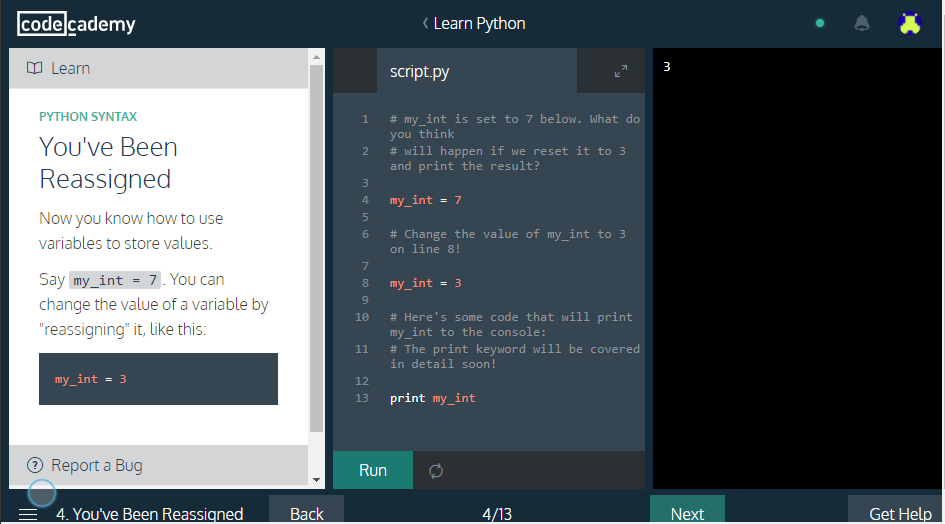
\includegraphics[]{codeacademy.png}
    }
    \caption[Codeacademy Python kurzus egyik feladata]{Codeacademy Python kurzus egyik feladata (forrás: \url{https://www.codecademy.com})}
    \label{fig:codeacademy}
\end{figure}

Az előzőleg felsoroltakkal szemben a Codeacademy nem nyílt forráskódú rendszer, így saját igényekre szabni nem lehet.

\section{Coursera}

A Coursera (\url{https://www.coursera.org/}), hasonlón az előző pontban részletezett Codeacademy rendszeréhez, egy teljeskörű, nem nyílt forráskódú eLearning rendszer. Itt is lehetőségünk van ingyenesen is tanulni, azonban ez korlátozásokat rejt magában. Ezt választva számítanunk kell rá, hogy nem férünk hozzá a kurzus minden tartalmához, de a tananyagok jelentős részét így is megtekinthetjük.

A Coursera a kurzusai megalkotásához együttműködik számos egyetemmel és egyéb szervezettel, melynek köszönhetően az oktatóanyagok magas színvonalúak. 2017. októberében a weboldal 2200 kurzusa volt elérhető a 28 millió regisztrált felhasználója számára.

\section{Dokeos}

A Dokeos (\url{https://www.dokeos.com}) az előzőekhez hasonló eLearning rendszer, melynek a Community Edition változata nyílt forráskódú. Ez a válozat több, mint 20 nyelven készült el a közösségi fejlesztés és fordítás eredményeképpen. Bárki szabadon használhatja, módosíthatja, testreszabhatja, futtathatja saját szervergépen, ezzel saját szolgáltatást indítva. A Dokeos eLearning Suite változata további szolgáltatásokat tartalmaz a Community Editon-höz képest, de ez már nem nyílt forráskódú. Ennek következtében ez csak a hivatalos oldalán érhető el fizetés ellenében.

A talált információk és vélemények alapján a programozási feladatok magas fokú támogatottsága nem megoldott a rendszerben. Emellett a Moodle több szempontból is egy jobb rendszernek tűnik:  jobban skálázódik és szélesebb körű oktatási támogatással rendelkezik, melynek köszönhetően sokkal inkább megfelel az egyedi igényeknek. \cite{DokeosVsMoodle}

\section{Összefoglalás}

A felsorolt nyílt forráskódú rendszerek egy általános megoldást biztosítanak az internetes oktatásra. Ezek legfőbb tulajdonságait \aref{table:elearning}. táblázat összegzi. Az általános megoldások biztosításának következtében a programozás specifikus feladatok létrehozása körülményesebb, illetve kevésbé személyre szabott lehet a létező moduloktól függően. Ezen okok adják a JPorta létjogosultságát, mivel az egy programozás orientált szemléletű, de mégis általános megoldást próbál nyújtani a felmerülő igényekre, melyeket a tervezési fázisban az oktatókkal közösen határozták meg.

\begin{table}[hp]
    \begin{tabularx}{\textwidth}{X|c|c|c|c|c|c}
                                            & Moodle     & ATutor     & edX        & Codeacademy & Coursera     & Dokeos     \\\hline
        Nyílt forráskód                     & \checkmark & \checkmark & \checkmark & X           & X            & \checkmark \\\hline
        Technológia                         & PHP        & PHP        & Python     &             &              & PHP        \\\hline
        Telefon támogatás                   & \checkmark & \checkmark & \checkmark & X           & \checkmark   & \checkmark \\\hline
        Kínált kurzusok                     & \checkmark & X          & \checkmark & \checkmark  & \checkmark   & X          \\\hline
        Egyedi kurzus                       & \checkmark & \checkmark & \checkmark & X           & X            & \checkmark \\\hline
        Automatikusan ellenőrződő feladatok & \checkmark & \checkmark & \checkmark & \checkmark  & \checkmark   & \checkmark \\\hline
        Feladatok időzítése                 & \checkmark & \checkmark & \checkmark & \checkmark  & \checkmark   & \checkmark \\\hline
        Egyéb beadandó feladatok            & \checkmark & \checkmark & \checkmark & \checkmark  & \checkmark   & \checkmark \\\hline
        Programozási feladatok              & \checkmark & X          & \checkmark & \checkmark  & \checkmark   & X \\\hline
        Dokumentum megosztás                & \checkmark & \checkmark & \checkmark & \checkmark  & \checkmark   & \checkmark \\\hline
        Fórum támogatás                     & \checkmark & \checkmark & \checkmark & \checkmark  & \checkmark   & \checkmark \\\hline
        Chat funkció                        & \checkmark & \checkmark & \checkmark & \checkmark  & \checkmark   & \checkmark \\\hline
        Szerepkörök (felhasználó, oktató, stb.) 
                                            & \checkmark & \checkmark & \checkmark & \checkmark  & \checkmark   & \checkmark \\\hline
        Egyetemi tárgyakhoz ideális         & \checkmark & \checkmark & \checkmark & X           & X            & \checkmark \\\hline
    \end{tabularx}
    \caption{eLearning rendszerek összegzés}				
    \label{table:elearning}
\end{table}